% Chương 4: Kết quả thực nghiệm

\chapter{Kết quả thực nghiệm}

\label{Chapter4}

%----------------------------------------------------------------------------------------

\section{Kết quả phân đoạn -- Benchmark 4 mô hình}

\subsection{Thiết lập thực nghiệm}

Bốn kiến trúc được huấn luyện và đánh giá độc lập trên cùng bộ dữ liệu LGG, sử dụng thư viện SMP \cite{Yakubovskiy2019} với encoder pretrained trên ImageNet. Để tối ưu ngưỡng phân loại, mỗi mô hình thực hiện grid search trên tập validation, sau đó áp dụng Test-Time Augmentation (TTA) khi đánh giá cuối. Bảng~\ref{tab:model_configs} tóm tắt cấu hình riêng của từng mô hình:

\begin{table}[h!]
    \centering
    \caption{Cấu hình thực nghiệm của bốn mô hình được đánh giá.}
    \label{tab:model_configs}
    \resizebox{\textwidth}{!}{%
    \begin{tabular}{l l r r r l}
        \toprule
        \tabhead{Mô hình} & \tabhead{Encoder} & \tabhead{Kích thước ảnh} & \tabhead{Epochs} & \tabhead{Ngưỡng} \\
        \midrule
        U-Net (SMP)   &  & $256\times256$ & 36 & 0.725 \\
        U-Net (SMP)   & ResNet-50       & $384\times384$ & 45 & 0.730  \\
        U-Net++ (SMP) & EfficientNet-B2 & $256\times256$ & 62 & 0.500 \\
        ResUNet (SMP) & ResNet-34       & $256\times256$ & 60 & 0.450 \\
        \bottomrule
    \end{tabular}}
\end{table}

\subsection{Bảng benchmark so sánh}

\begin{table}[h!]
    \centering
    \caption{Kết quả thực nghiệm.}
    \label{tab:benchmark}
    \resizebox{\textwidth}{!}{%
    \begin{tabular}{l l r r r r r}
        \toprule
        Kiến trúc & Encoder & Dice & IoU & Precision & Recall & F1-Score \\
        \midrule
        U-Net (SMP)   & -                & 0.7794 & 0.6385 & 0.8666 & 0.7081 & 0.7760 \\
        U-Net (SMP)   & ResNet-50       & 0.7766 & 0.6348 & 0.8396 & 0.7225 & 0.7780 \\
        U-Net++ (SMP) & EfficientNet-B2 & 0.7992 & 0.6656 & 0.8946 & 0.7220 & 0.7766 \\
        \textbf{ResUNet (SMP)} & \textbf{ResNet-34} & \textbf{0.8846} & \textbf{0.7931} & \textbf{0.8929} & \textbf{0.8764} & \textbf{0.8846} \\
        \bottomrule
    \end{tabular}}
\end{table}

\textbf{ResUNet + ResNet-34 vượt trội hoàn toàn} so với ba kiến trúc còn lại trên mọi độ đo:  DiCe 0.8846 cao hơn U-Net tới $+10.5\%$ ; IoU 0.7931 cao hơn U-net $+15.5\%$; Recall 0.8764 cho thấy tỷ lệ bỏ sót khối u rất thấp. Đây là kết quả đáng chú ý vì ResNet-34 là encoder nhẹ nhưng kiến trúc ResUNet tận dụng residual connections để học đặc trưng biên sắc nét hơn.

\subsection{Lịch sử huấn luyện}

\begin{figure}[htbp]
    \centering
    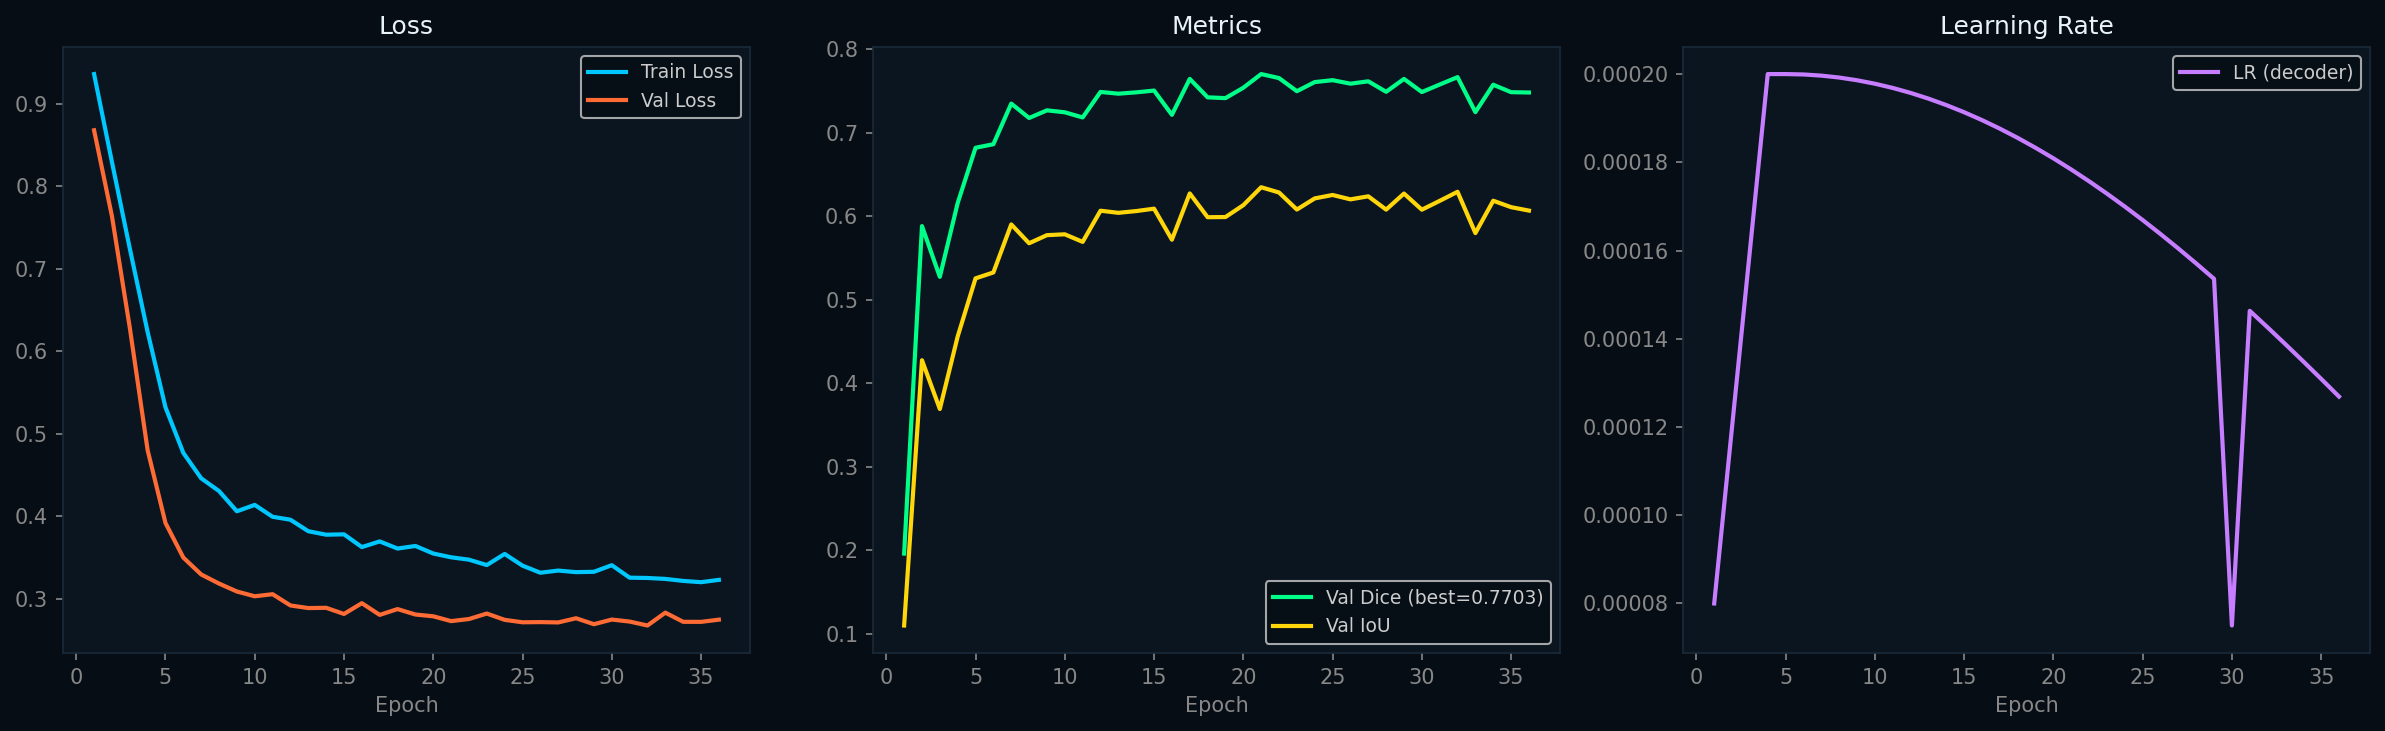
\includegraphics[width=\textwidth]{Figures/Gallery/m1_uneteffb2_history.png}
    \caption{Lịch sử huấn luyện U-Net (EfficientNet-B2).}
    \label{fig:hist_unet_effb2}
\end{figure}

\begin{figure}[htbp]
    \centering
    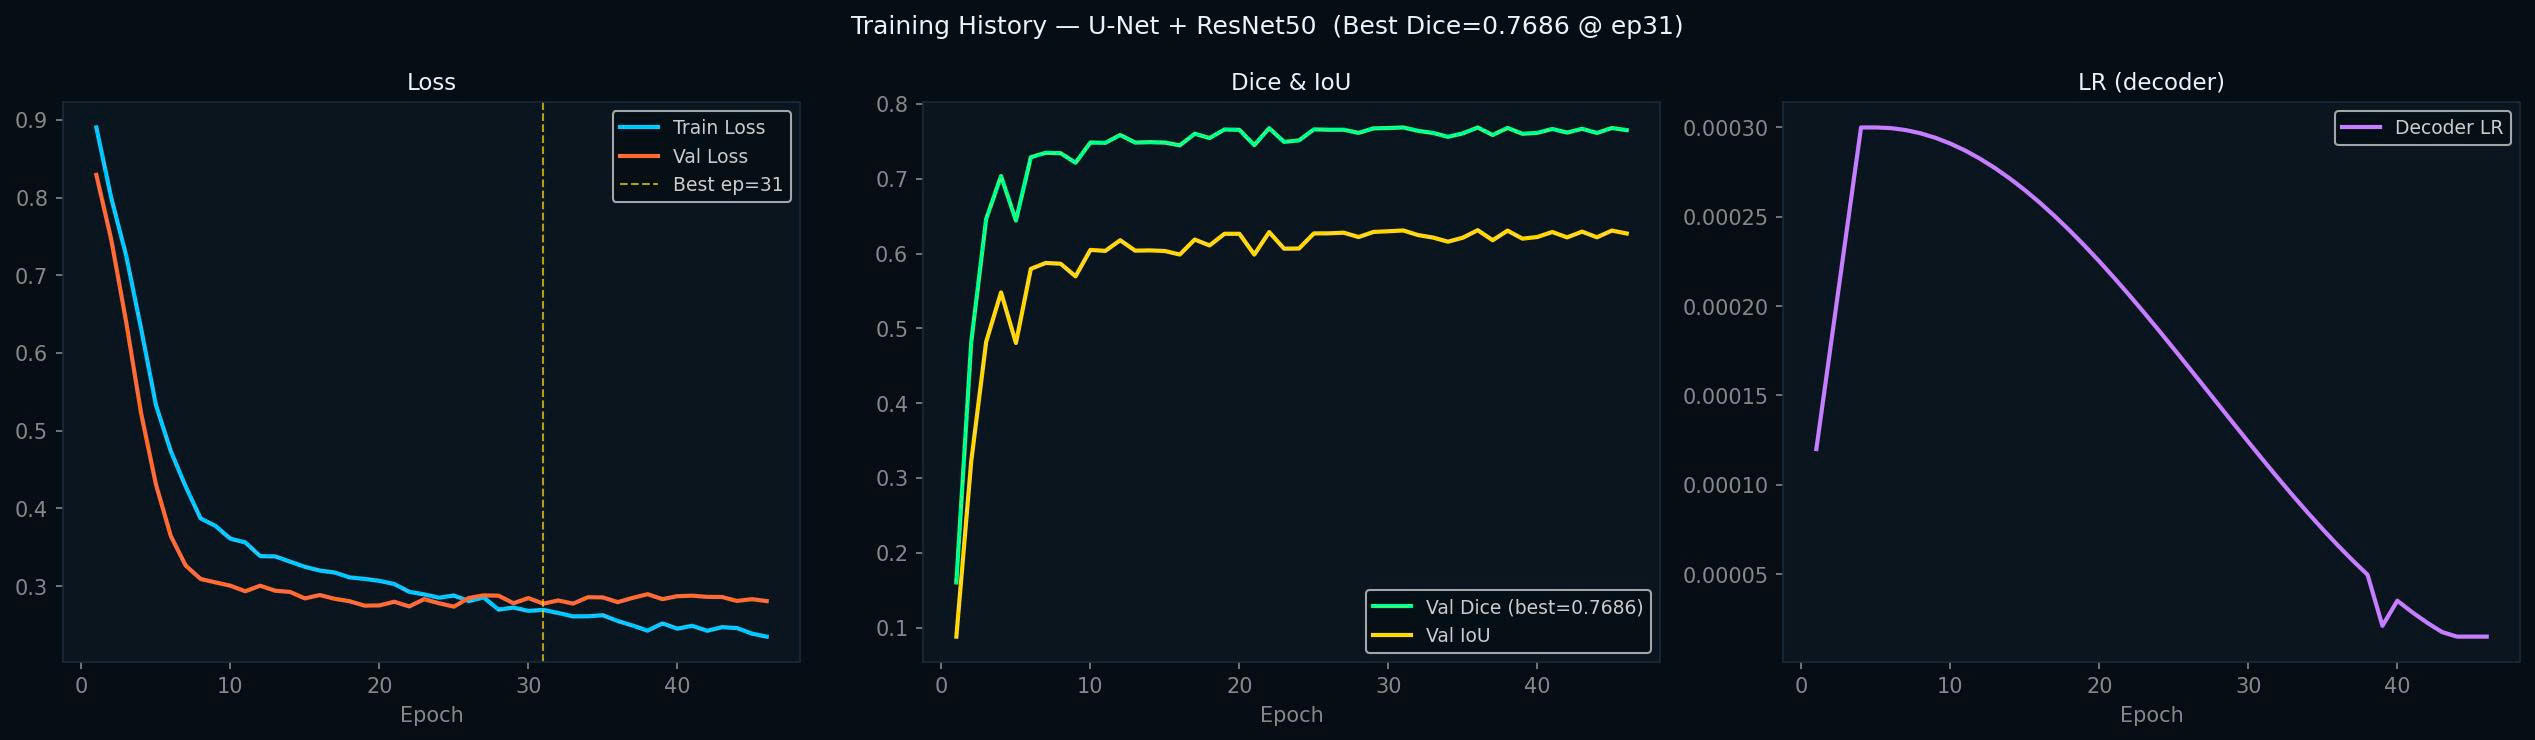
\includegraphics[width=\textwidth]{Figures/Gallery/m2_unetresnet50_history.jpg}
    \caption{Lịch sử huấn luyện U-Net (ResNet-50).}
    \label{fig:hist_unet_resnet50}
\end{figure}

\FloatBarrier

\begin{figure}[htbp]
    \centering
    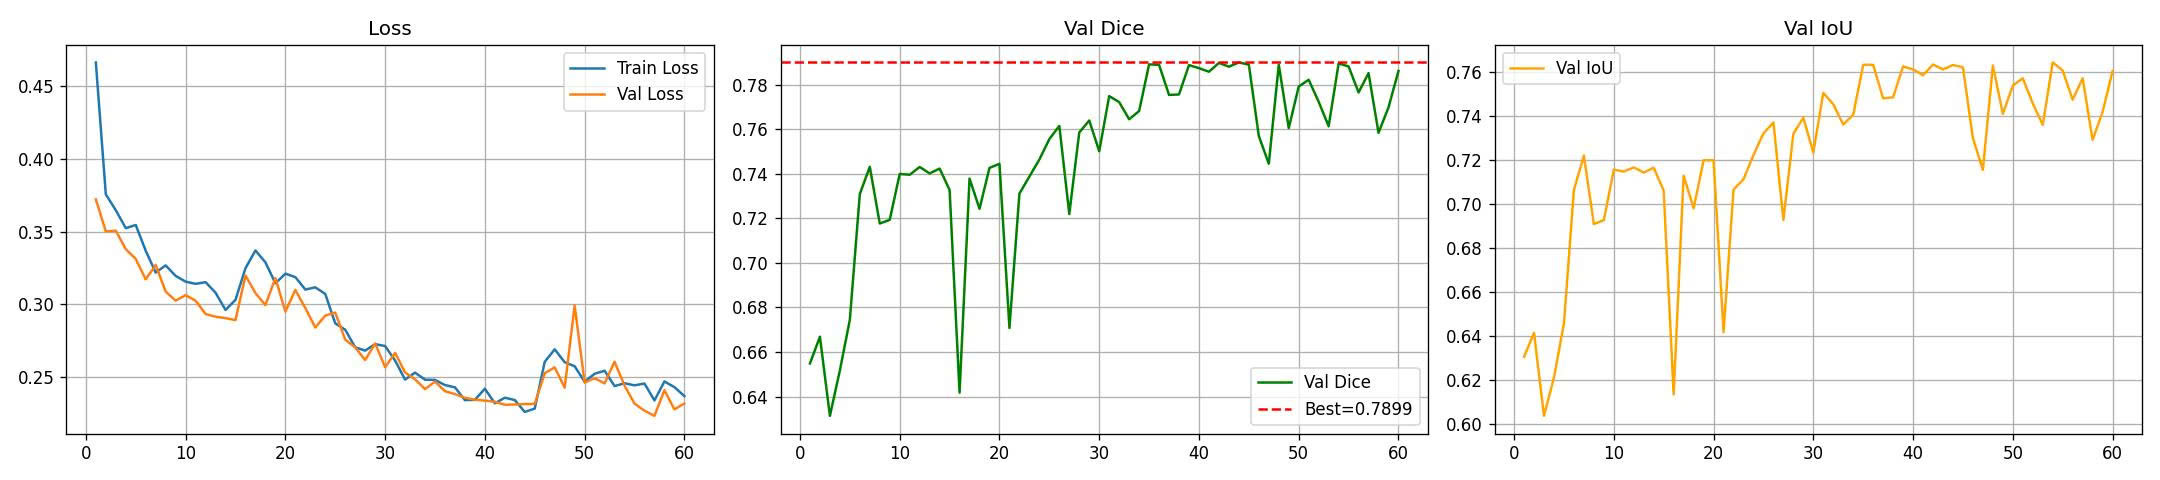
\includegraphics[width=\textwidth]{Figures/Gallery/m3_unetppeffb2_history.jpg}
    \caption{Lịch sử huấn luyện U-Net++ (EfficientNet-B2).}
    \label{fig:hist_unetpp_effb2}
\end{figure}

\begin{figure}[htbp]
    \centering
    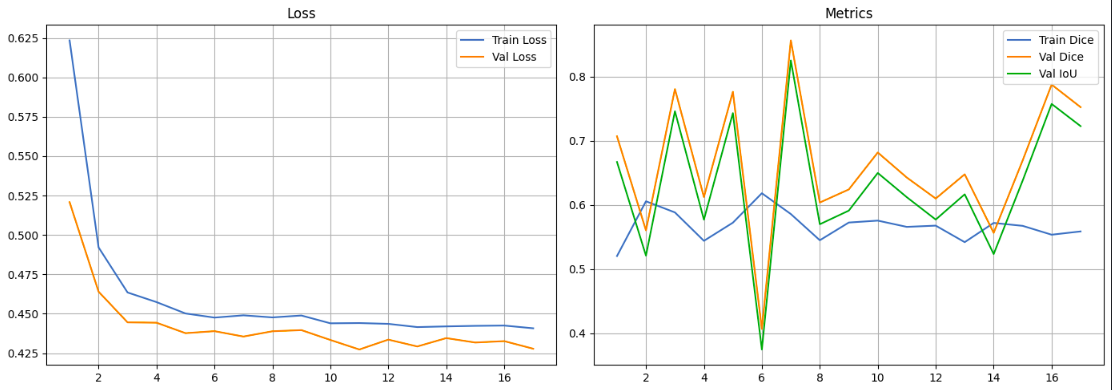
\includegraphics[width=\textwidth]{Figures/Chapter/Chapter6.png}
    \caption{Lịch sử huấn luyện ResUNet (ResNet-34).}
    \label{fig:hist_resunet}
\end{figure}

\FloatBarrier

\subsection{Kết quả dự đoán định tính}

\begin{figure}[H]
    \centering
    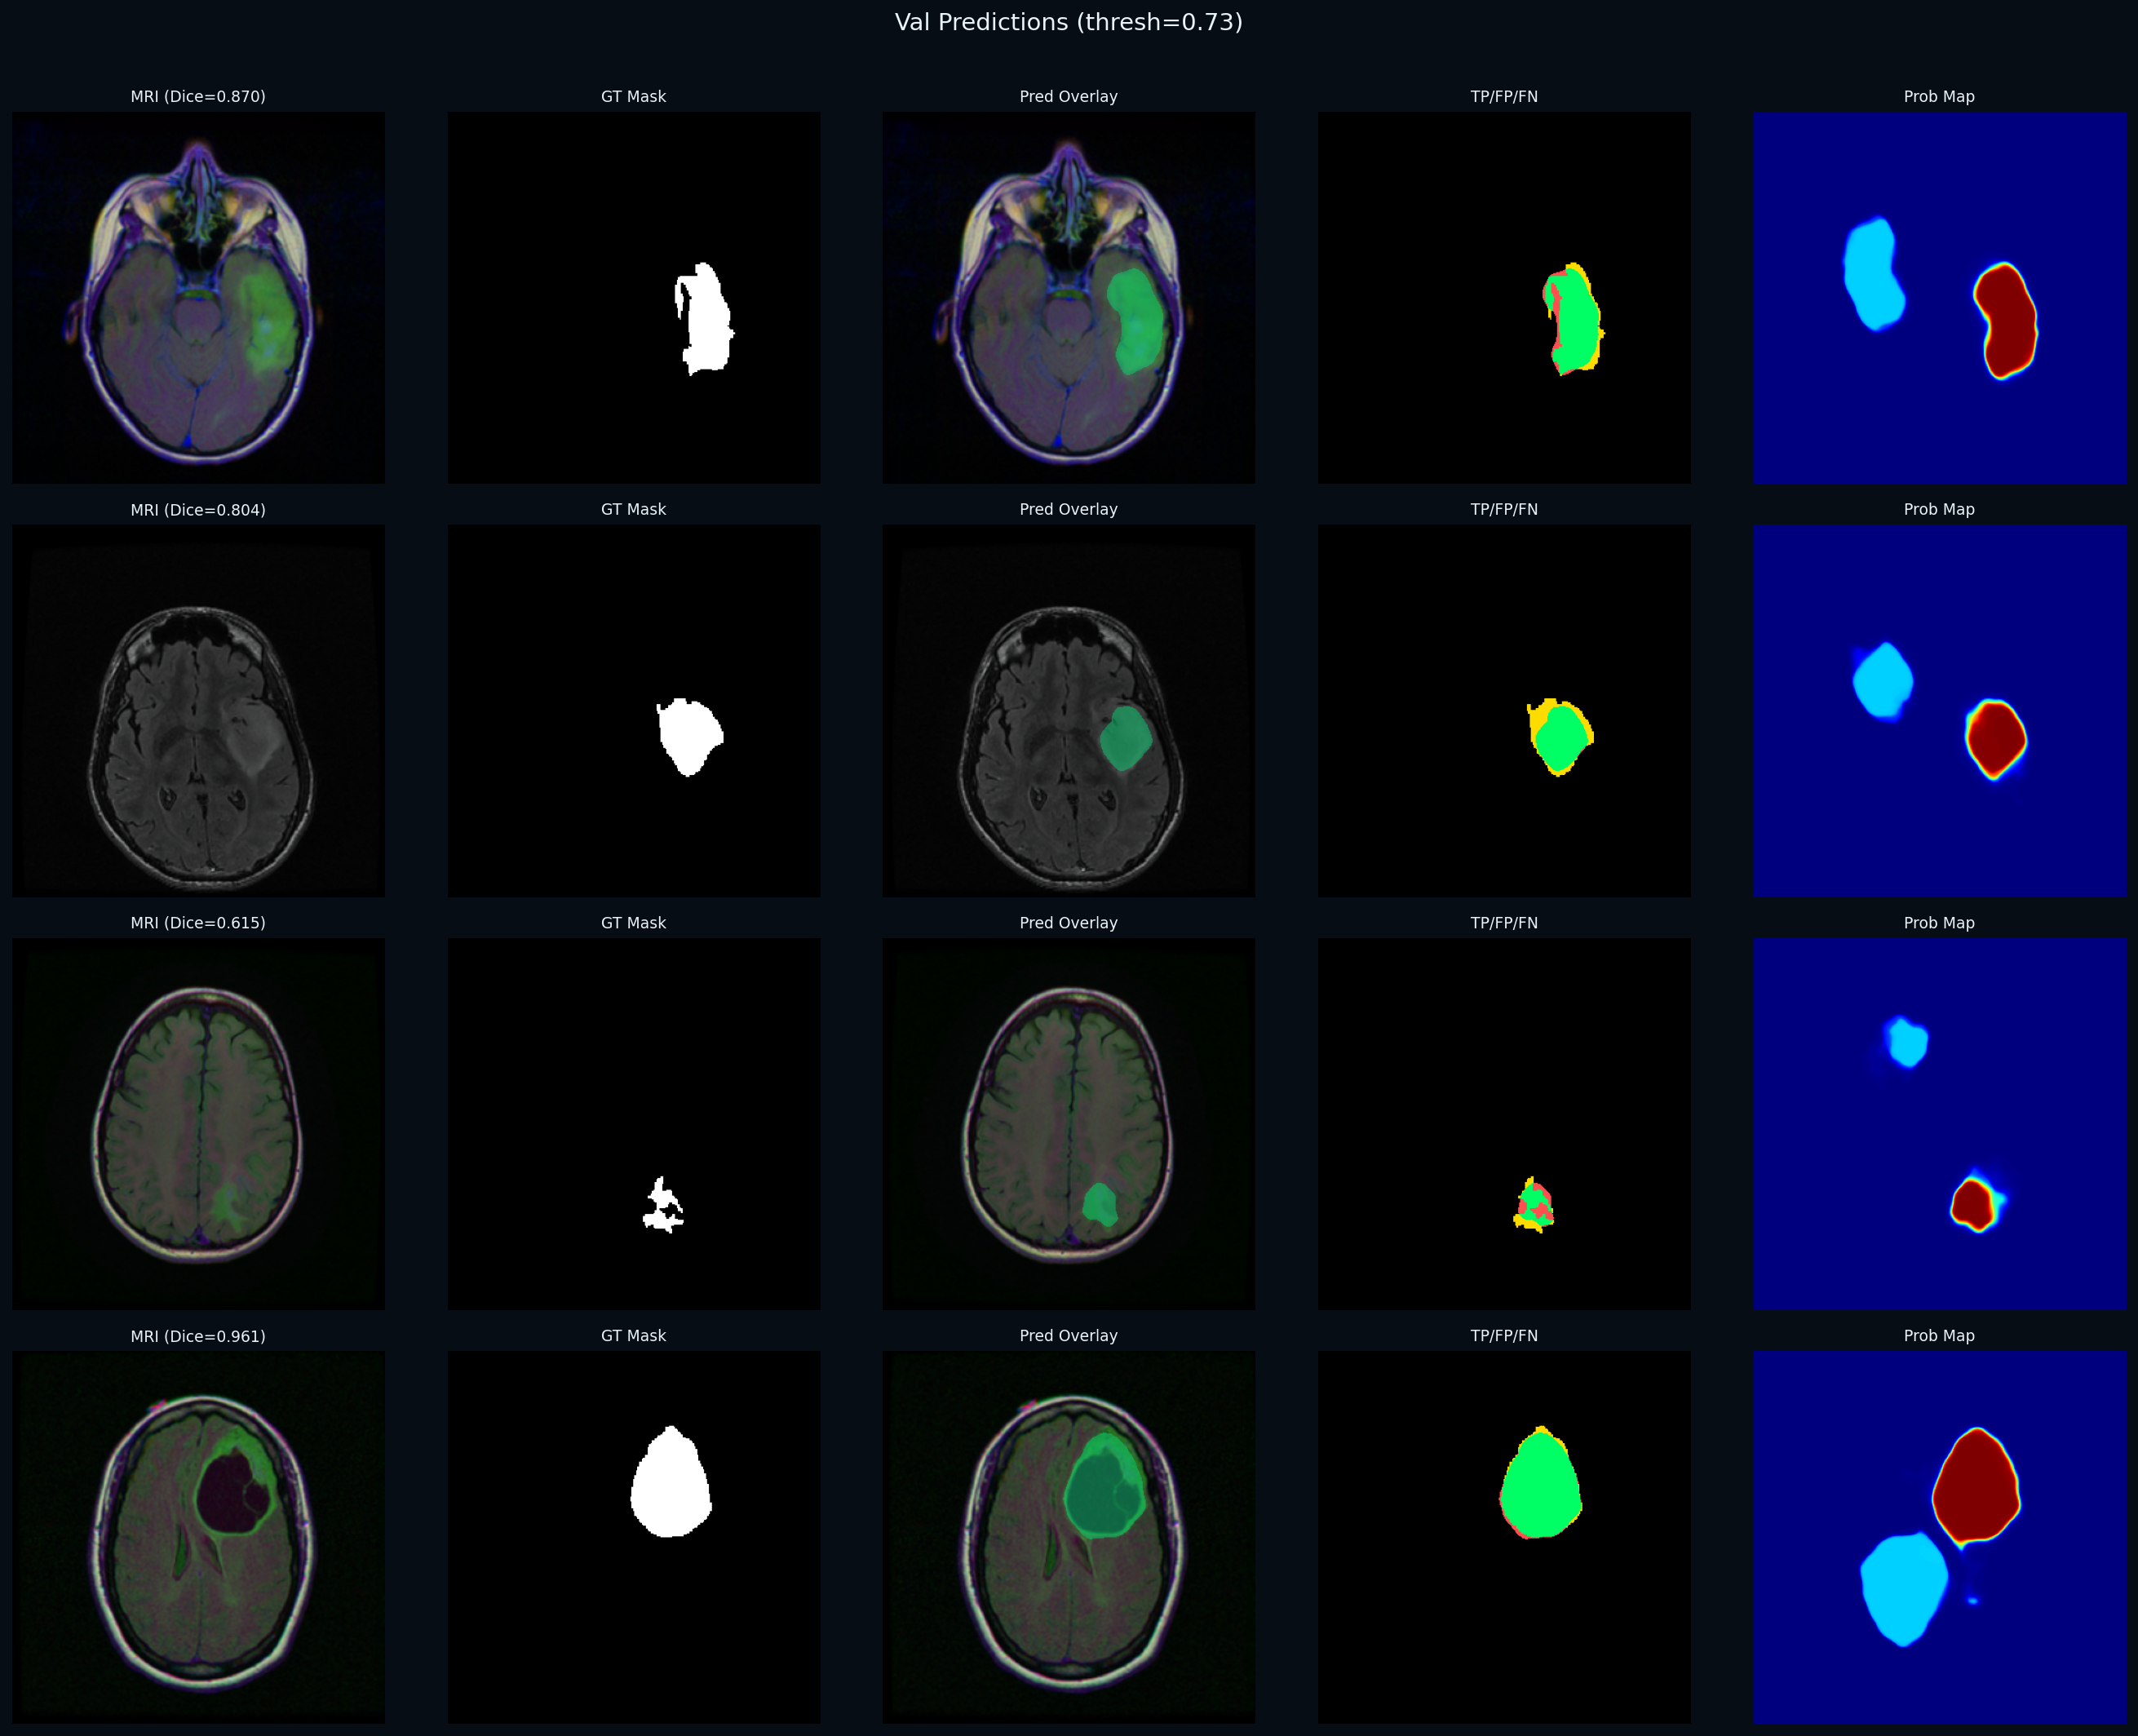
\includegraphics[width=0.85\textwidth,height=0.22\textheight,keepaspectratio]{Figures/Gallery/m1_uneteffb2_preds.png}
    \caption{Mẫu dự đoán của U-Net (EfficientNet-B2).}
\end{figure}

\begin{figure}[H]
    \centering
    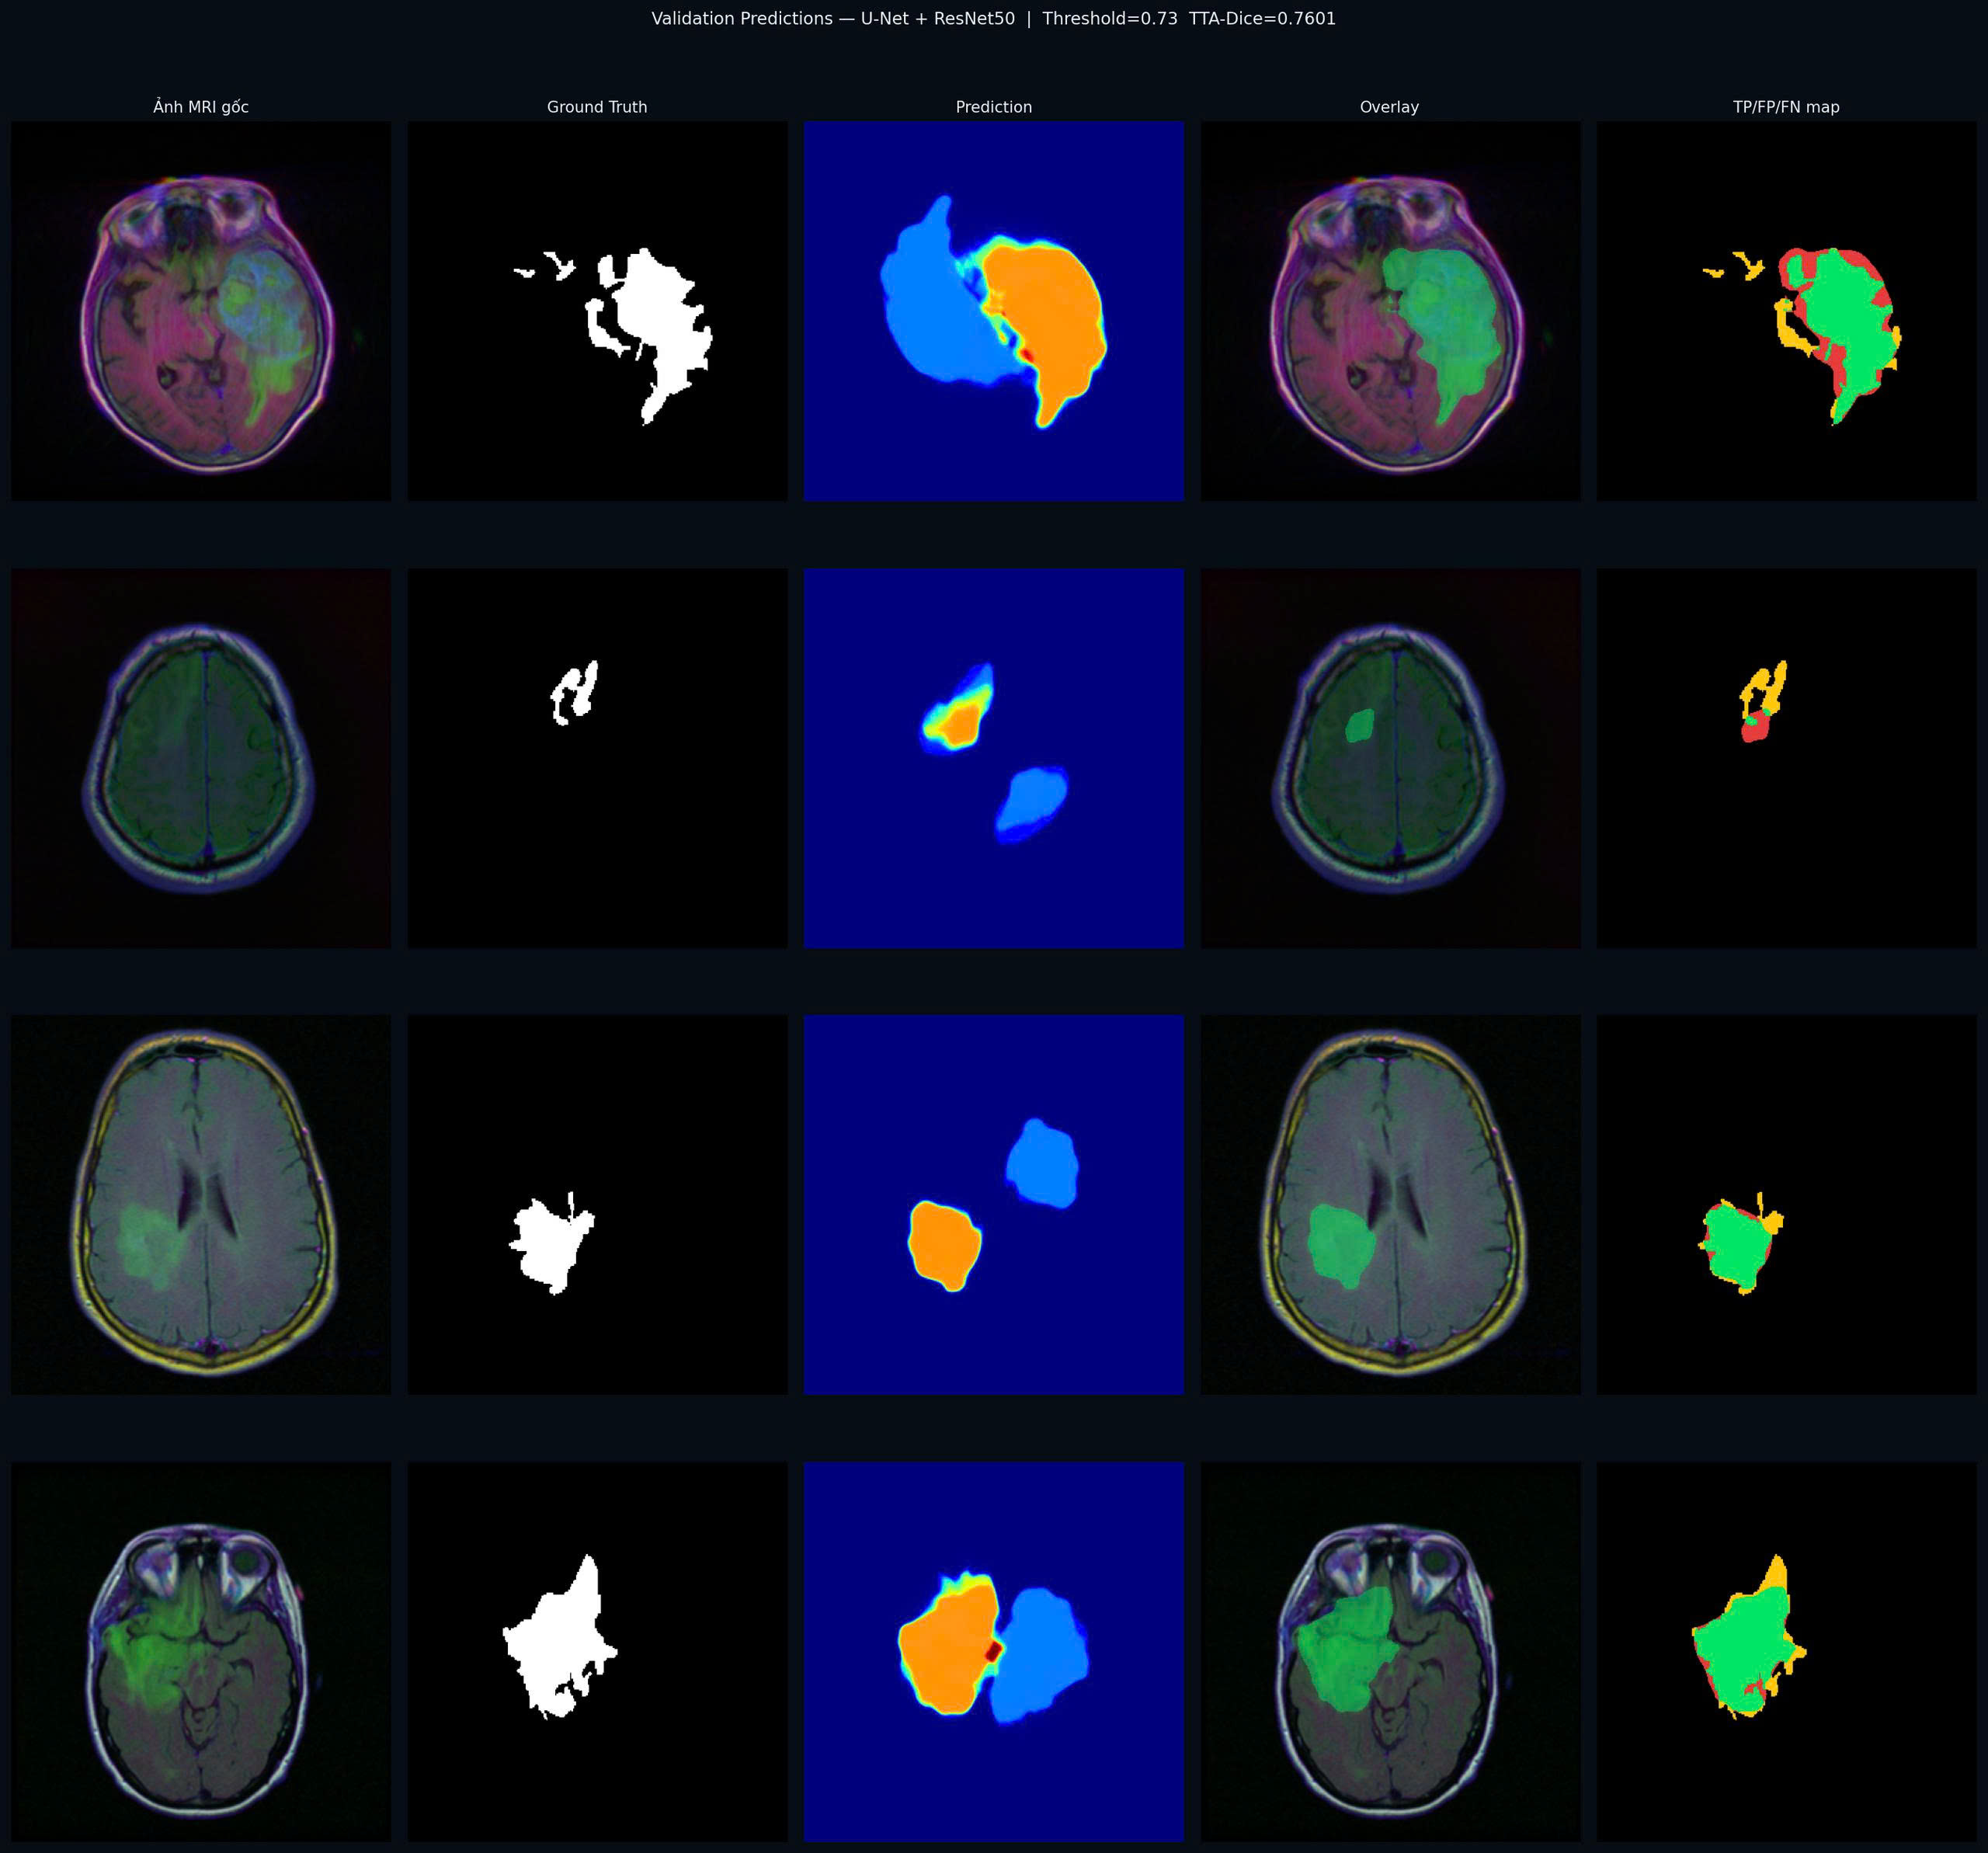
\includegraphics[width=0.85\textwidth,height=0.22\textheight,keepaspectratio]{Figures/Gallery/m2_unetresnet50_preds.jpg}
    \caption{Mẫu dự đoán của U-Net (ResNet-50).}
\end{figure}

\begin{figure}[H]
    \centering
    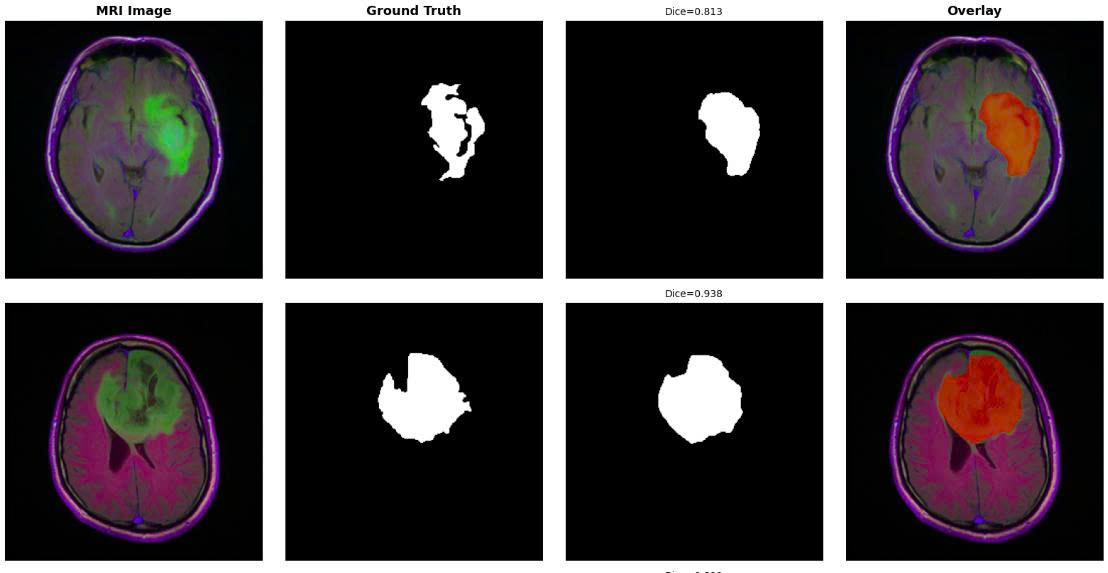
\includegraphics[width=0.85\textwidth,height=0.22\textheight,keepaspectratio]{Figures/Gallery/m3_unetppeffb2_preds.jpg}
    \caption{Mẫu dự đoán của U-Net++ (EfficientNet-B2).}
\end{figure}

\begin{figure}[H]
    \centering
    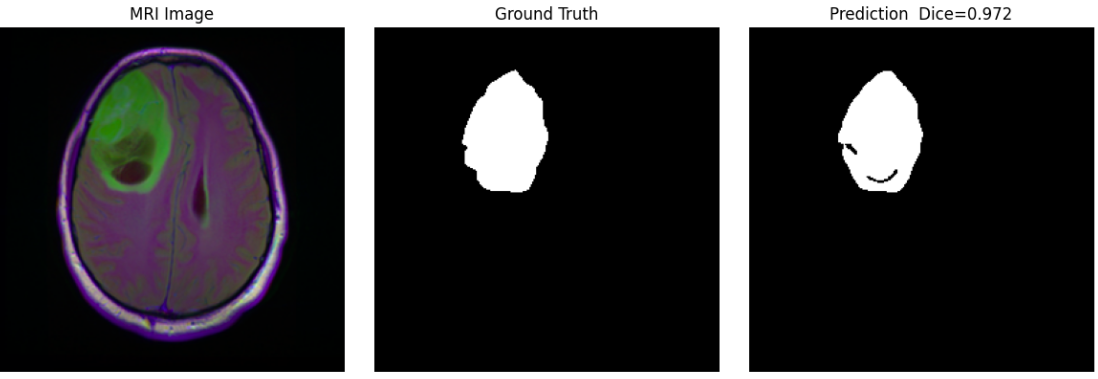
\includegraphics[width=0.85\textwidth,height=0.22\textheight,keepaspectratio]{Figures/Chapter/Chapter7.png}
    \caption{Mẫu dự đoán của ResUNet (ResNet-34).}
\end{figure}
\subsection{Phân tích và lựa chọn mô hình}

Dựa trên kết quả benchmark đầy đủ, \textbf{ResUNet + ResNet-34} được lựa chọn là mô hình triển khai chính trong hệ thống BrainSeg-XAI vì các lý do sau:

\begin{sloppypar}
\begin{enumerate}
    \item \textbf{DiCe cao nhất (0.8846):} Vượt tất cả các kiến trúc còn lại với biên độ lớn ($+$10.5 điểm tuyệt đối so với U-Net). Đây là số liệu trên tập test thực tế, không phải validation.
    \item \textbf{Recall vượt trội (0.8764):} Trong chẩn đoán u não, bỏ sót khối u (FN) là lỗi nghiêm trọng hơn báo dương giả (FP). Recall 0.8764 đảm bảo hệ thống phát hiện được phần lớn vùng bệnh lý.
    \item \textbf{IoU 0.7931 -- ngưỡng lâm sàng có ý nghĩa:} IoU $> 0.75$ thường được coi là mức phân đoạn tốt trong y tế. Ba mô hình còn lại đều dưới ngưỡng này.
    \item \textbf{Encoder nhẹ, inference nhanh:} ResNet-34 có ít tham số hơn EfficientNet-B2 và ResNet-50, phù hợp triển khai trên CPU không có GPU.
    \item \textbf{Ngưỡng auto-tuned 0.45:} Ngưỡng thấp hơn 0.5 giúp mô hình có xu hướng phát hiện nhiều vùng hơn, ưu tiên Recall -- chiến lược hợp lý về mặt lâm sàng.
\end{enumerate}
\end{sloppypar}

\section{Trực quan hóa Grad-CAM}

Bản đồ Grad-CAM trực quan hóa vùng ảnh ảnh hưởng đến quyết định phân đoạn. Phân tích định tính cho thấy:

\begin{itemize}
    \item Đối với ảnh có khối u rõ, bản đồ nhiệt tập trung chính xác vào vùng tăng tín hiệu tương ứng với khối u.
    \item Đối với ảnh không có khối u, Grad-CAM phân tán đều trên nhiều vùng, không có điểm nóng rõ ràng -- xác nhận mô hình không ``bịa đặt'' khối u giả.
    \item Một số trường hợp Grad-CAM kích hoạt vào cả vùng não khỏe mạnh lân cận khối u, phản ánh việc mô hình sử dụng ngữ cảnh không gian khi đưa ra quyết định.
\end{itemize}

Đây là hành vi mong đợi: Grad-CAM không chỉ hiển thị vùng khối u mà hiển thị vùng ảnh hưởng đến quyết định phân đoạn toàn cục.

\section{Phân tích bộ máy luật rủi ro}

Trên tập kiểm thử, phân bố điểm rủi ro phản ánh đặc điểm bộ dữ liệu LGG:
\begin{itemize}
    \item Phần lớn trường hợp rơi vào mức \textit{Thấp} hoặc \textit{Trung bình}, phù hợp với đặc tính u độ thấp (LGG) vốn phát triển chậm và ít xâm lấn hơn so với GBM.
    \item Các trường hợp được phân loại \textit{Cao} hoặc \textit{Rất cao} thường là khối u lớn, đa ổ hoặc có dịch chuyển đường giữa đáng kể.
    \item Quy tắc đóng góp điểm nhiều nhất trong dữ liệu LGG: R6 (diện tích tuyệt đối) và R2 (bất đối xứng hình dạng).
\end{itemize}

Điều quan trọng cần lưu ý là hệ thống luật không được xác thực lâm sàng chính thức và chỉ mang tính hỗ trợ tham khảo.

\section{Kiểm thử hệ thống end-to-end}

Hệ thống được kiểm thử bằng cách khởi động backend FastAPI và gọi API trực tiếp. Dưới đây là kết quả thực tế thu được từ endpoint \texttt{POST /api/v1/predict} ở chế độ demo (không có file weights huấn luyện):

\begin{table}[h!]
    \centering
    \caption{Kết quả kiểm thử hệ thống end-to-end trên CPU.}
    \label{tab:e2e_test}
    \begin{tabular}{l l l}
        \toprule
        \tabhead{Kịch bản} & \tabhead{Kết quả} & \tabhead{HTTP Status} \\
        \midrule
        File ảnh PNG hợp lệ          & JSON đầy đủ, pipeline chạy   & 200 OK \\
        File không phải ảnh          & Lỗi, thông báo rõ ràng       & 400 \\
        File $> 20$ MB               & Từ chối                      & 413 \\
        Không có file weights        & Demo mode, pipeline đầy đủ   & 200 OK \\
        \midrule
        \texttt{GET /api/v1/health}  & \texttt{\{"status":"ok"\}}   & 200 OK \\
        \bottomrule
    \end{tabular}
\end{table}

\subsection{Ví dụ response API thực tế}

Kết quả JSON trả về từ một request thực (demo mode, trọng số ngẫu nhiên) có cấu trúc như sau. Trường \texttt{features} chứa vector đặc trưng hình thái đầy đủ, và trường \texttt{risk} chứa đánh giá rủi ro có cấu trúc:

\begin{lstlisting}[style=plaintext, caption={Vi du response JSON tu POST /api/v1/predict (truong base64 da luoc bo)}]
{
  "features": {
    "tumor_detected":      true,
    "tumor_area_px":       20884,
    "tumor_area_cm2":      183.55,
    "occupancy_ratio":     31.87,
    "num_regions":         1073,
    "shape_irregularity":  0.9976,
    "compactness":         0.0024,
    "boundary_complexity": 72.0239,
    "midline_shift":       false,
    "location":            "thuy dinh/thai duong, trung tam",
    "centroid_x":          127.9,
    "centroid_y":          133.7
  },
  "risk": {
    "risk_level":  "Rat cao",
    "risk_score":  100,
    "severity":    "Nguy kich",
    "risk_color":  "#ff2d55",
    "fired_rules": [
      "Ty le chiem vung nao rat cao (31.87% > 20%)",
      "Hinh dang khoi u rat bat doi xung (irr=1.00)",
      "Duong bien khoi u rat phuc tap (complexity=72.0)",
      "Phat hien nhieu vung khoi u (1073 vung)",
      "Dien tich khoi u rat lon (183.55 cm2)"
    ],
    "recommendations": [
      "KHAN CAP: Can nhap vien va can thiep ngay lap tuc",
      "Can can thiep phau thuat khan cap",
      "Sinh thiet de xac dinh tinh ac tinh",
      "Chi dinh PET-CT de danh gia do xam lan"
    ],
    "explanation": "He thong phan tich 5 dac trung y khoa va
      kich hoat 5 co nguy co. Diem nguy co: 100/100.
      Phan loai: Nguy kich."
  }
}
\end{lstlisting}

Lưu ý: response trên là từ demo mode (trọng số ngẫu nhiên) nên các giá trị đặc trưng không phản ánh thực tế lâm sàng. Với model đã huấn luyện trên bộ dữ liệu LGG, kết quả phân đoạn sẽ khớp với vùng tín hiệu bất thường thực tế trên ảnh MRI.



%----------------------------------------------------------------------------------------
\section{Hạn chế hiện tại}
%----------------------------------------------------------------------------------------

\textbf{1. Phạm vi dữ liệu hạn hẹp.}
Hệ thống được huấn luyện và đánh giá trên bộ dữ liệu LGG thuần nhất. Hiệu suất trên dữ liệu GBM, u di căn hay các loại u khác chưa được kiểm chứng.

\textbf{2. Xử lý ảnh 2D đơn lẻ.}
Hệ thống chỉ xử lý từng lát cắt MRI riêng lẻ, không tận dụng thông tin không gian 3D từ toàn bộ sequence, giới hạn khả năng ước lượng thể tích khối u.

\textbf{3. Bộ máy luật chưa được xác thực lâm sàng.}
Các ngưỡng và trọng số điểm trong bộ máy luật được xác định theo tài liệu tham khảo, chưa trải qua xác thực prospective với bác sĩ chuyên khoa.

\textbf{4. Thiếu đánh giá calibration.}
Mô hình chưa được kiểm tra độ hiệu chỉnh xác suất: xác suất sigmoid đầu ra có thực sự phản ánh tần suất dự đoán đúng không?

\textbf{5. Phụ thuộc chất lượng ảnh đầu vào.}
Hệ thống chưa có cơ chế phát hiện ảnh chất lượng kém (nhiễu cao, thiếu tương phản) và chưa thực hiện chuẩn hóa cường độ theo từng thiết bị MRI.

%----------------------------------------------------------------------------------------
\section{Hướng phát triển}
%----------------------------------------------------------------------------------------

\subsection{Mở rộng sang phân đoạn 3D}

Bước phát triển tự nhiên là xử lý toàn bộ sequence MRI dưới dạng khối 3D. Các kiến trúc như 3D U-Net hoặc nnU-Net cho phép học đặc trưng không gian ba chiều, cải thiện độ chính xác phân đoạn và tính được thể tích khối u trực tiếp.

\subsection{Đa phương thức và đa chuỗi xung}

Kết hợp đồng thời nhiều chuỗi xung MRI (T1, T2, FLAIR, T1-Gd) như chuẩn của cuộc thi BraTS \cite{Menze2015} cho phép khai thác tương quan thông tin, cải thiện độ chính xác phân đoạn các tiểu vùng (tumor core, enhancing tumor, edema).

\subsection{Xác thực lâm sàng}

Để hướng tới ứng dụng thực tế:
\begin{itemize}
    \item Xác thực prospective các ngưỡng trong bộ máy luật với bác sĩ chuyên khoa thần kinh.
    \item Đánh giá inter-rater agreement giữa chú thích của hệ thống và bác sĩ.
    \item Tuân thủ quy định y tế như FDA 510(k) hoặc CE Mark tùy thị trường mục tiêu.
\end{itemize}

\subsection{Tích hợp PACS và giao diện mở rộng}

Tích hợp với hệ thống PACS (Picture Archiving and Communication System) giúp nhận ảnh DICOM trực tiếp từ thiết bị MRI. Giao diện có thể mở rộng hỗ trợ MPR viewer (xem lát cắt 3D), xuất báo cáo PDF và lưu trữ kết quả theo bệnh nhân.

\subsection{Cải thiện khả năng giải thích}

Ngoài Grad-CAM, có thể tích hợp thêm SHAP để giải thích đóng góp từng đặc trưng hình thái vào điểm rủi ro; attention maps từ kiến trúc transformer; và uncertainty quantification (Monte Carlo Dropout) để ước tính độ không chắc chắn của dự đoán.

%----------------------------------------------------------------------------------------
\section{Kết luận chung}
%----------------------------------------------------------------------------------------

BrainSeg-XAI thể hiện rằng việc xây dựng một hệ thống AI y tế \textit{có thể giải thích được} là khả thi với các công nghệ nguồn mở hiện có. Hệ thống không chỉ tạo ra mặt nạ phân đoạn mà còn cung cấp cơ chế giải thích đa lớp: Grad-CAM ở cấp độ pixel, đặc trưng hình thái ở cấp độ vùng, và đánh giá rủi ro có cấu trúc ở cấp độ lâm sàng. Đây là hướng tiếp cận phù hợp với xu hướng phát triển của AI y tế: không thay thế bác sĩ mà trang bị cho họ công cụ phân tích mạnh mẽ và minh bạch hơn để đưa ra quyết định lâm sàng chính xác.
